\documentclass[pdflatex,compress,mathserif]{beamer}

%\usetheme[dark,framenumber,totalframenumber]{ElektroITK}
\usetheme[darktitle,framenumber,totalframenumber]{ElektroITK}

\usepackage[utf8]{inputenc}
\usepackage[T1]{fontenc}
\usepackage{lmodern}
\usepackage[bahasai]{babel}
\usepackage{amsmath}
\usepackage{amsfonts}
\usepackage{amssymb}
\usepackage{graphicx}
\usepackage{multicol}

\newcommand*{\Scale}[2][4]{\scalebox{#1}{$#2$}}%

\title{PEMODELAN JARINGAN KOMUNIKASI}
\subtitle{VLANs - Virtual Local Area Networks}

\author{Tim Dosen Pengampu}

\begin{document}
	
\maketitle

\section{Campus Design - Access, Distribution and Core Layers}

\begin{frame}
	\frametitle{Campus Design - Access, Distribution and Core Layers}
	\begin{itemize}
		\item The campus LAN should be designed for scalability, performance and
security
		\item To aid in a best practice design process, the network topology is split
into access, distribution and core layers
		\item The layers have their own design principles and characteristics
	\end{itemize}
\end{frame}

\begin{frame}
	\frametitle{Campus Design – Access Layer}
	\begin{center}
		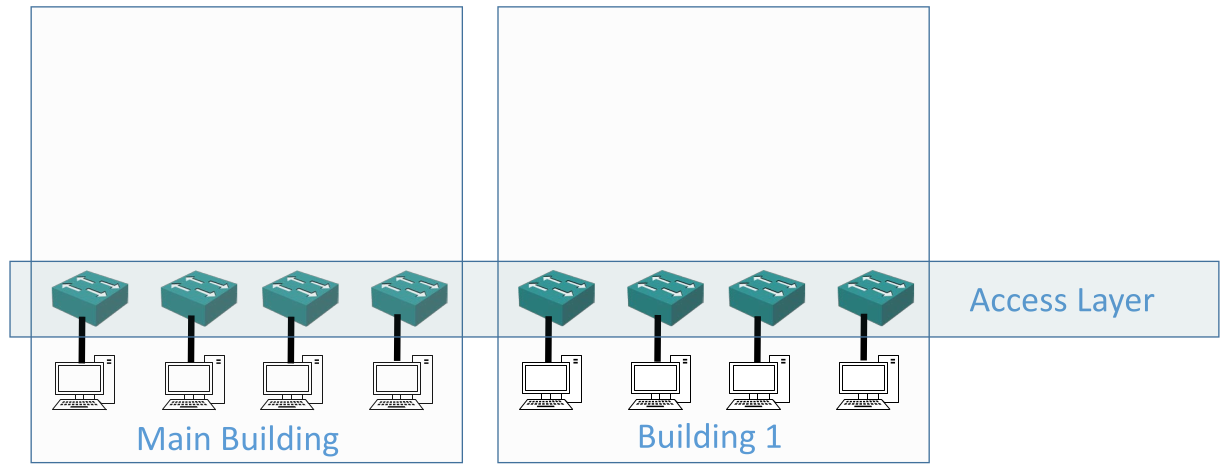
\includegraphics[width=\linewidth]{img/img01}
	\end{center}
\end{frame}

\begin{frame}
	\frametitle{The Access Layer}
	\begin{itemize}
		\item End hosts such as desktop computers, servers and IP phones connect
into the network at the access layer
		\item It is designed to have a high port count at an affordable cost
		\item Desktops typically have only one Network Interface Card (NIC) so they
connect into one switch or Wireless Access Point
		\item Servers will often have dual NICs and connect to a pair of redundant
switches
		\item Client access security measures are enabled at the Access Layer
	\end{itemize}
\end{frame}

\begin{frame}
	\frametitle{Campus Design - Distribution Layer}
	\begin{center}
		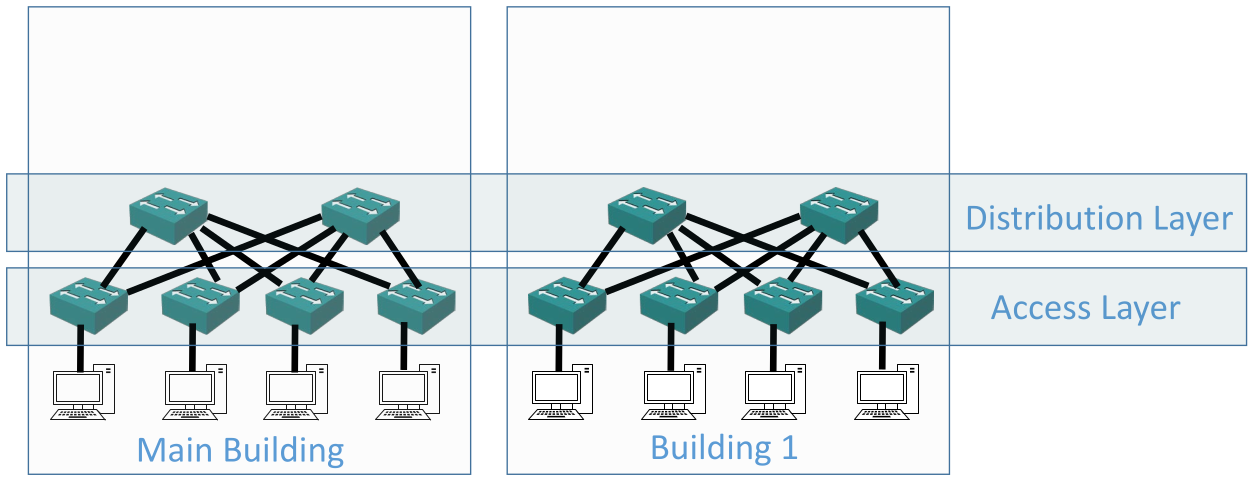
\includegraphics[width=\linewidth]{img/img02}
	\end{center}
\end{frame}

\begin{frame}
	\frametitle{The Distribution Layer}
	\begin{itemize}
		\item Access Layer switches uplink to Distribution Layer switches
		\item The Distribution Layer switches serve as an aggregation point for the
Access Layer and provide scalability
		\item Distribution Layer switches are typically deployed in redundant pairs,
with downstream Access Layer switches connected to both
		\item End hosts are not typically connected here
		\item Most software policy such as QoS is enabled at this layer
	\end{itemize}
\end{frame}

\begin{frame}
	\frametitle{Campus Design - Core Layer}
	\begin{center}
		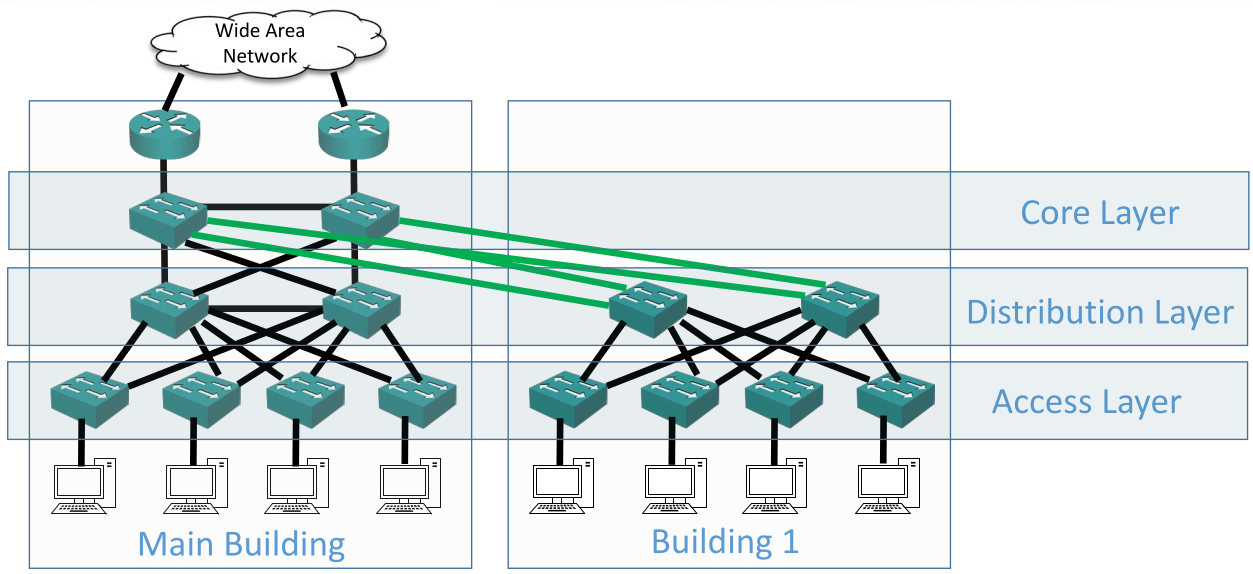
\includegraphics[width=\linewidth]{img/img03}
	\end{center}
\end{frame}

\begin{frame}
	\frametitle{The Core Layer}
	\begin{itemize}
		\item Distribution Layer switches uplink to Core Layer switches
		\item Core Layer switches are typically deployed in redundant pairs, with
downstream Distribution Layer switches connected to both
		\item Traffic between different parts of the campus travels through the core
so it is designed for speed and resiliency
		\item Software policy slows the switch down so should be avoided in the
Core Layer
	\end{itemize}
\end{frame}

\begin{frame}
	\frametitle{Collapsed Distribution and Core}
	\begin{itemize}
		\item Smaller campuses do not need the scalability of three separate layers
		\item In these cases a Collapsed Distribution and Core layer is used, where
the Distribution and Core layer functions are performed on the same
hardware device
	\end{itemize}
\end{frame}

\begin{frame}{Collapsed Distribution and Core}
	\begin{center}
		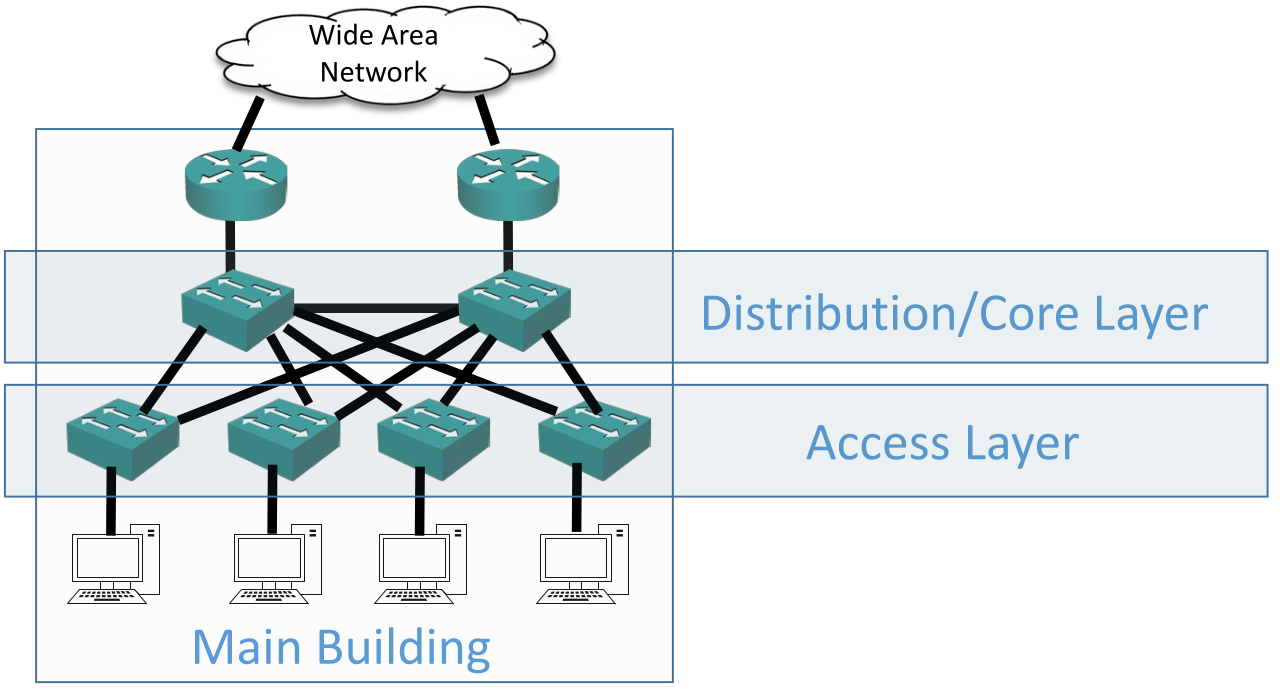
\includegraphics[width=\linewidth]{img/img04}
	\end{center}
\end{frame}

\section{Spine-Leaf Network Design}

\begin{frame}
	\frametitle{Traditional Campus Design}
	\begin{center}
		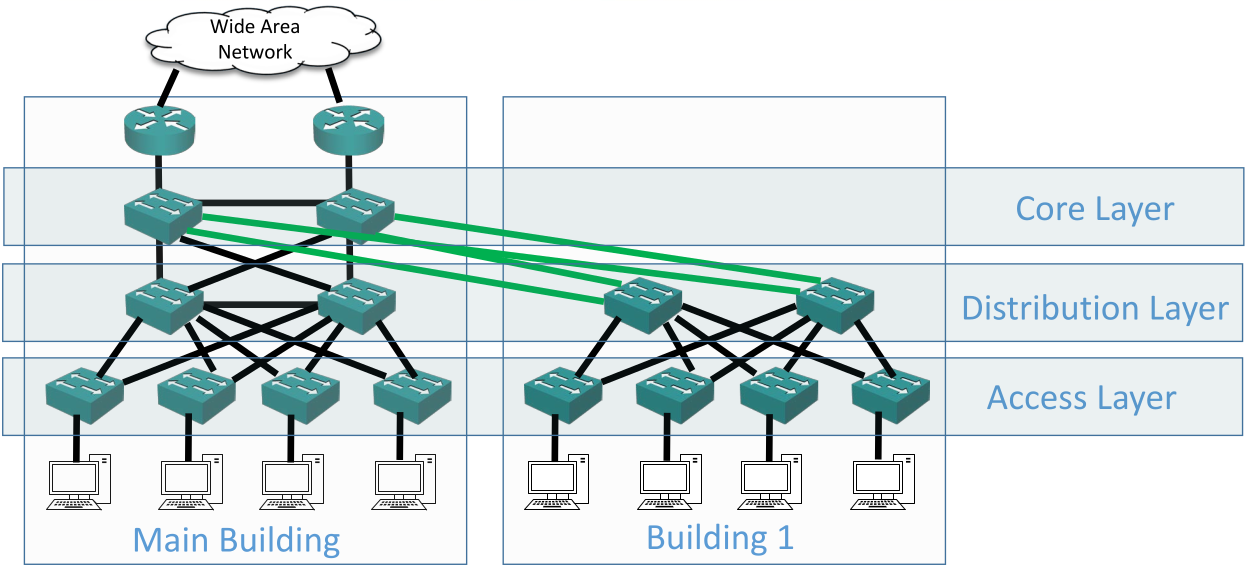
\includegraphics[width=\linewidth]{img/img05}
	\end{center}
\end{frame}

\begin{frame}{Traditional Campus Design}
	\begin{center}
		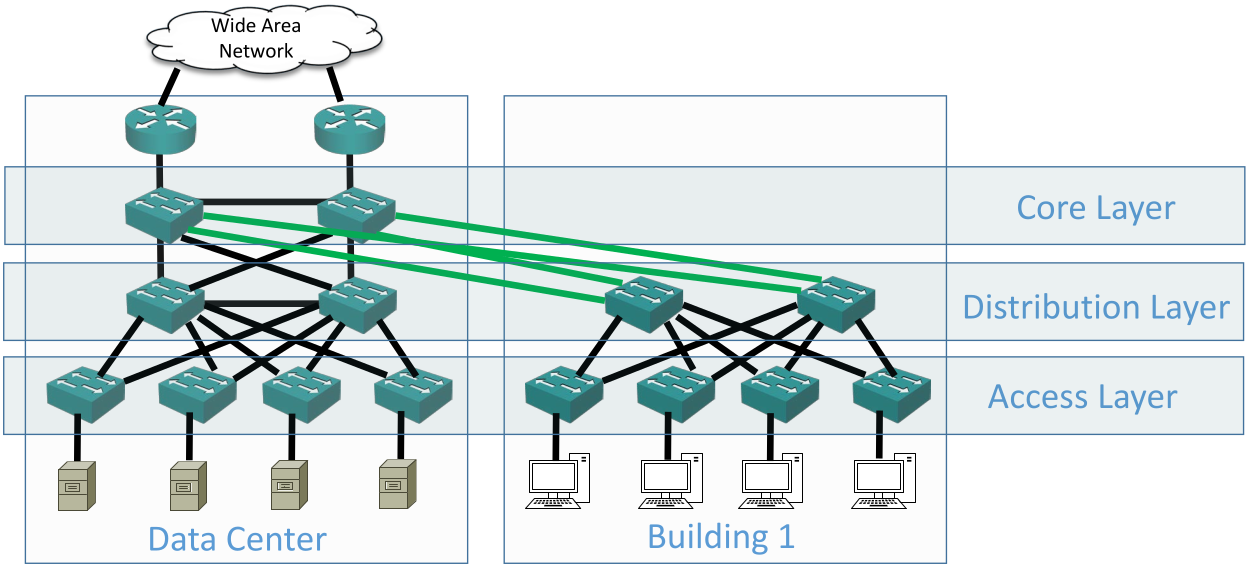
\includegraphics[width=\linewidth]{img/img06}
	\end{center}
\end{frame}

\begin{frame}
	\frametitle{Spine-Leaf Data Center Design}
	\begin{center}
		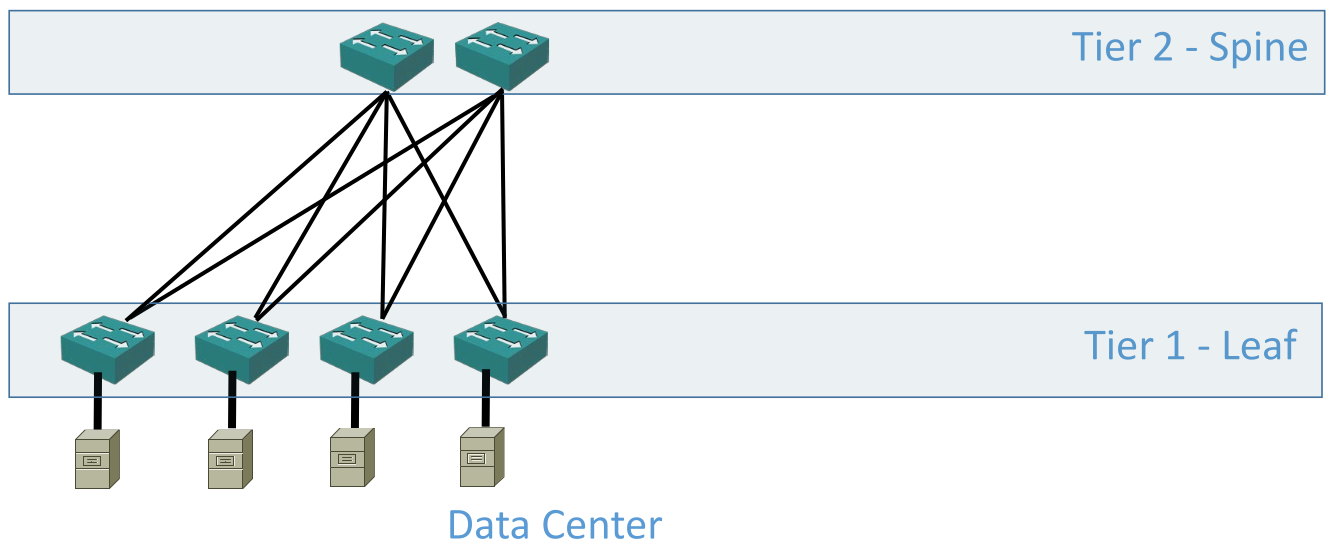
\includegraphics[width=\linewidth]{img/img07}
	\end{center}
\end{frame}

\begin{frame}{Spine-Leaf Data Center Design}
	\begin{center}
		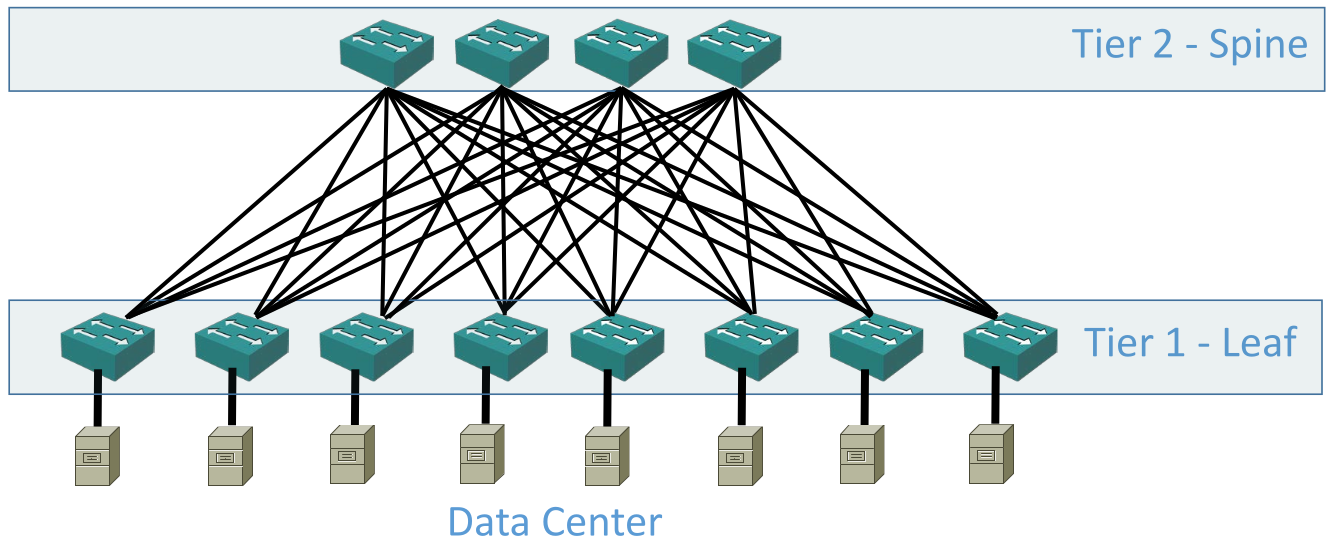
\includegraphics[width=\linewidth]{img/img08}
	\end{center}
\end{frame}

\section{Why we have VLANs}

\begin{frame}
	\frametitle{Router Operations}
	\begin{itemize}
		\item Routers operate at Layer 3 of the OSI stack
		\item Hosts in separate IP subnets must send traffic via a router to
communicate
		\item Security rules on routers or firewalls can be used to easily control what
traffic is allowed between different IP subnets at Layer 3
		\item Routers do not forward broadcast traffic by default
		\item They provide performance and security by splitting networks into
smaller domains at Layer 3
	\end{itemize}
\end{frame}

\begin{frame}
	\frametitle{Switch Operations}
	\begin{itemize}
		\item Switches operate at Layer 2 of the OSI stack
		\item They \textbf{do} forward broadcast traffic by default
		\item By default a campus switched network is one large broadcast domain
		\item Switches flood broadcast traffic everywhere, including between
different IP subnets
		\item This raises performance and security concerns
	\end{itemize}
\end{frame}

\begin{frame}
	\frametitle{LAN Networks}
	\begin{center}
		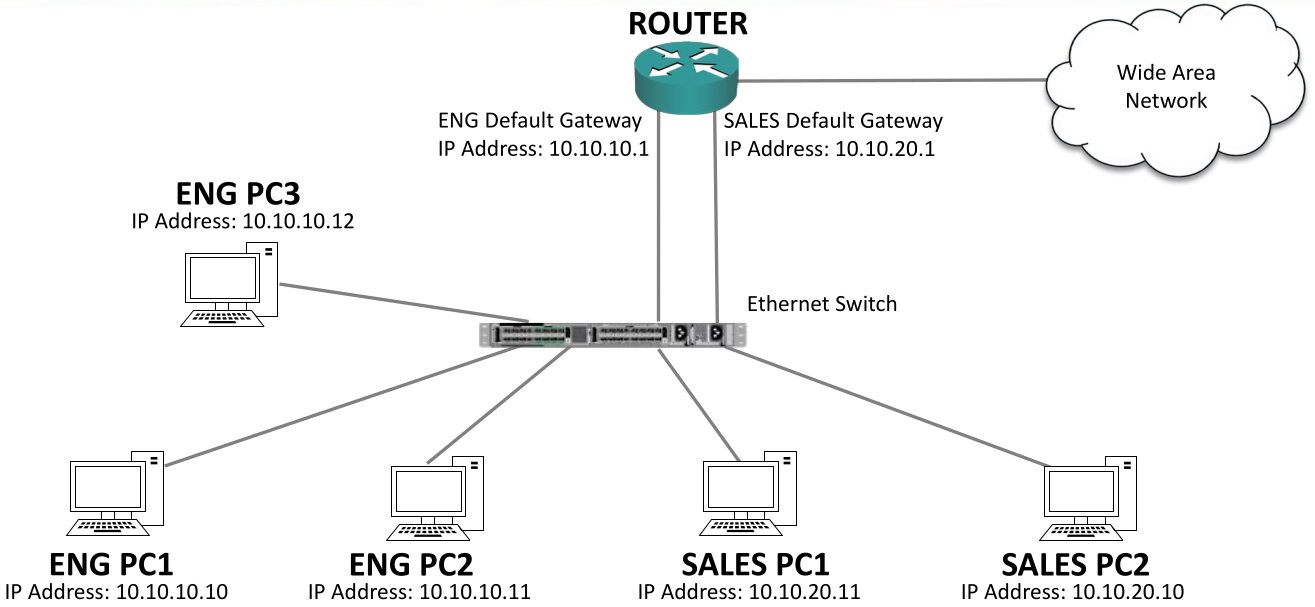
\includegraphics[width=\linewidth]{img/img09}
	\end{center}
\end{frame}

\begin{frame}
	\frametitle{Unicast Traffic within same IP subnet}
	\begin{center}
		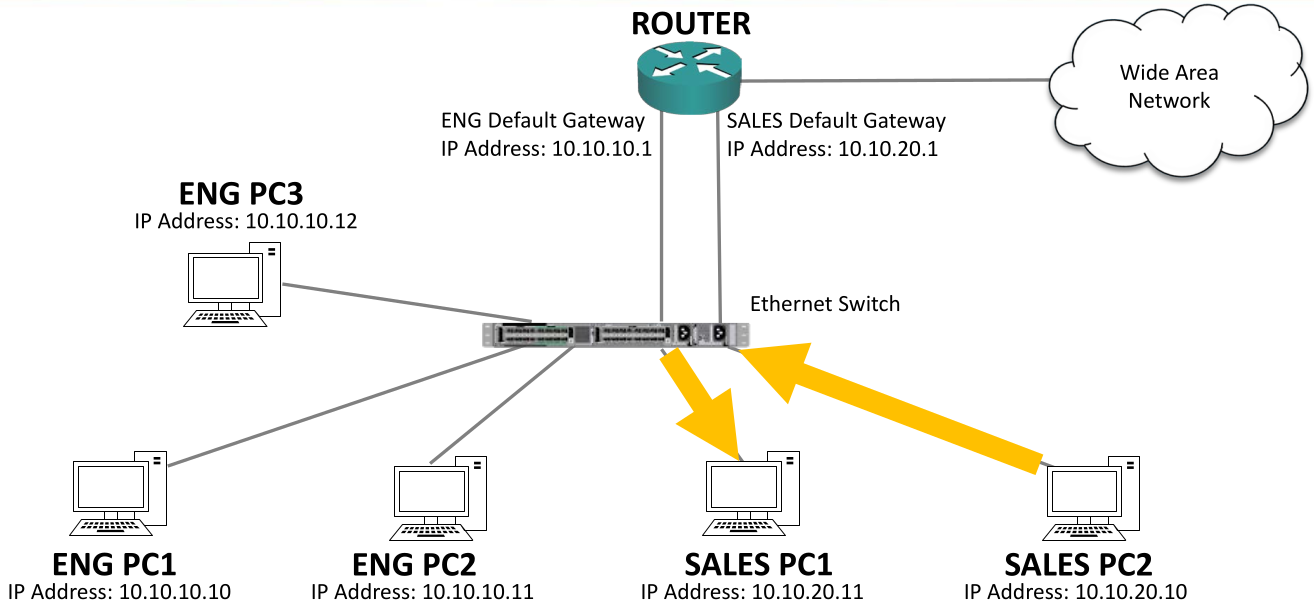
\includegraphics[width=\linewidth]{img/img10}
	\end{center}
\end{frame}

\begin{frame}
	\frametitle{Unicast Traffic between different IP subnets}
	\begin{center}
		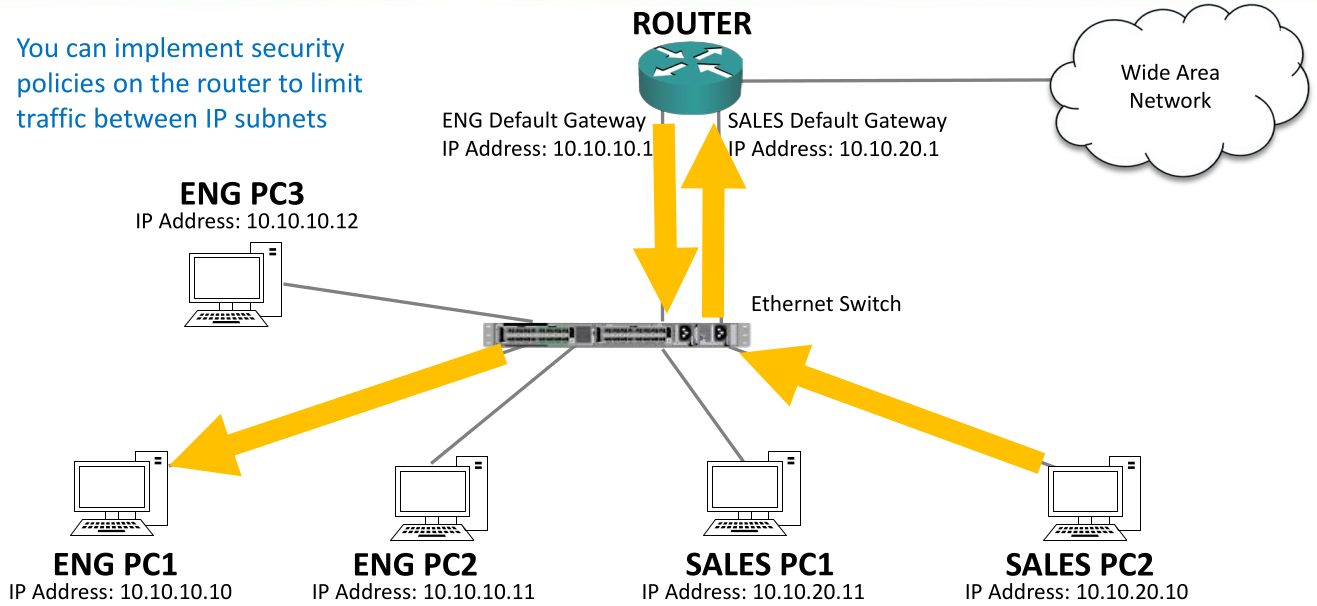
\includegraphics[width=\linewidth]{img/img11}
	\end{center}
\end{frame}

\begin{frame}
	\frametitle{Broadcast Traffic}
	\begin{center}
		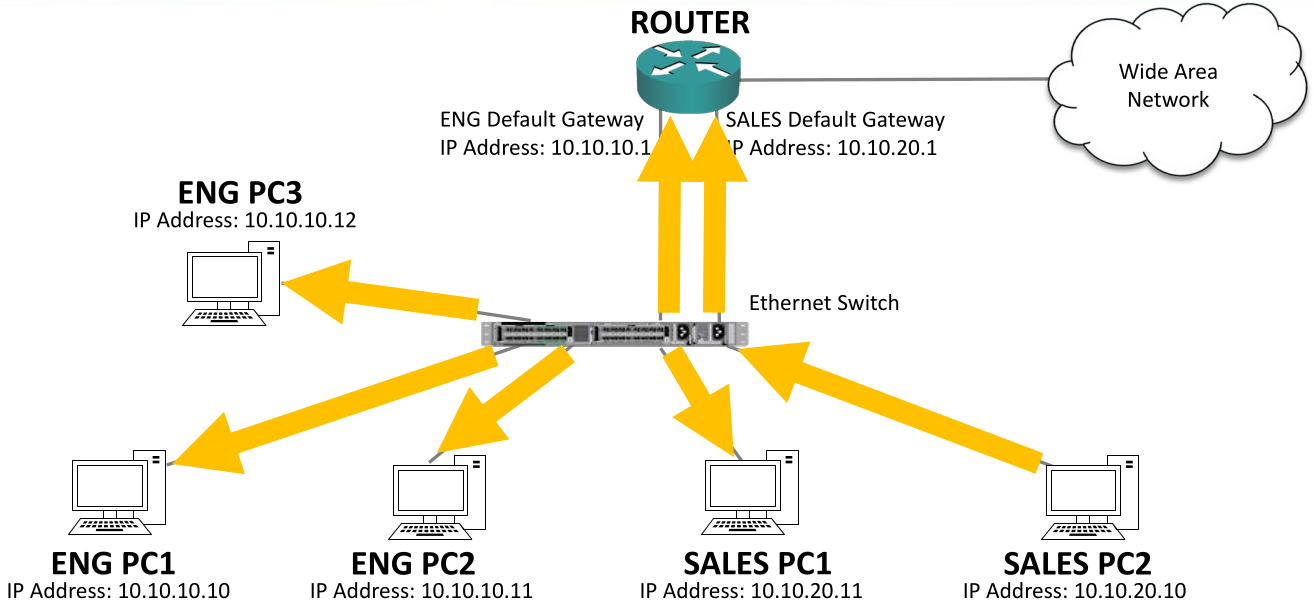
\includegraphics[width=\linewidth]{img/img12}
	\end{center}
\end{frame}

\begin{frame}
	\frametitle{The Problem}
	\begin{itemize}
		\item Switches flood broadcast traffic everywhere, including between
different IP subnets
		\item This affects security because the traffic bypasses router or firewall
Layer 3 security policies
		\item It affects performance because every end host has to process the
traffic
		\item It also affects performance by using bandwidth on links where the
traffic is not required
	\end{itemize}
\end{frame}

\begin{frame}
	\frametitle{Broadcast Traffic}
	\begin{center}
		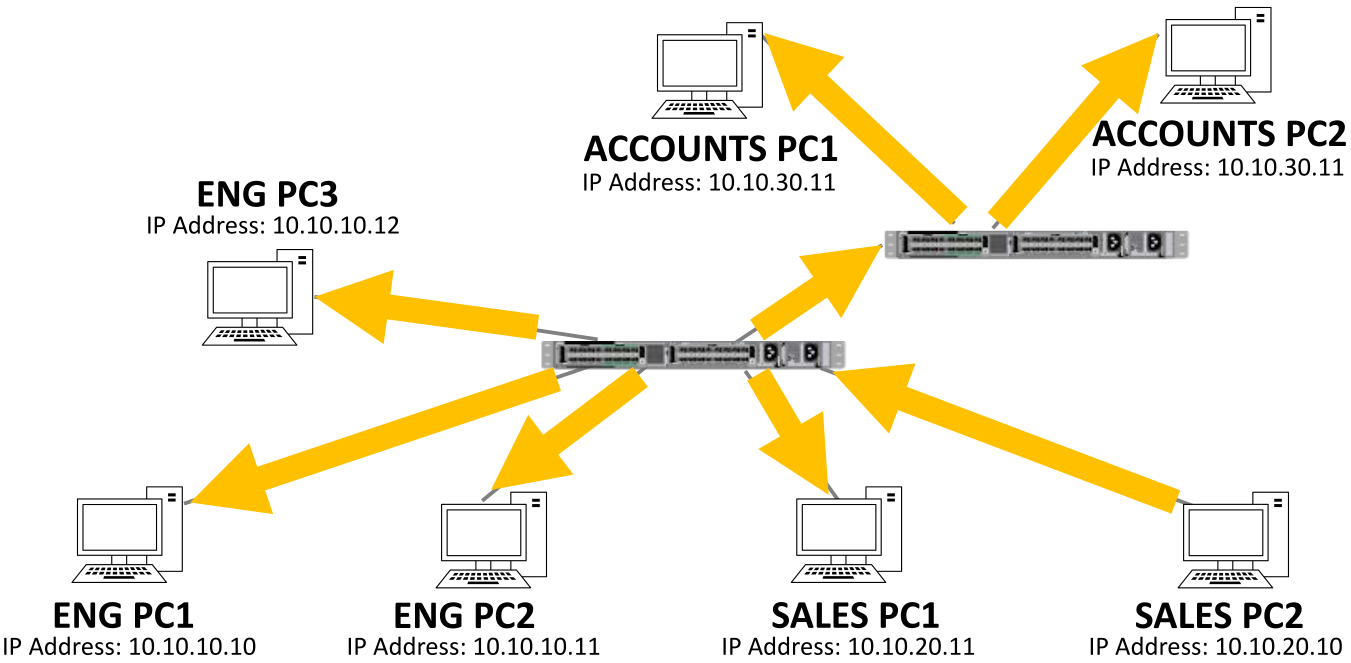
\includegraphics[width=\linewidth]{img/img13}
	\end{center}
\end{frame}

\begin{frame}
	\frametitle{VLAN Virtual Local Area Networks}
	\begin{itemize}
		\item We can increase performance and security in the LAN by implementing
VLANs on our switches
		\item VLANs segment the LAN into separate broadcast domains at Layer 2
		\item There is typically a one-to-one relationship between an IP subnet and
a VLAN
	\end{itemize}
\end{frame}

\begin{frame}{VLAN Virtual Local Area Networks}
	\begin{center}
		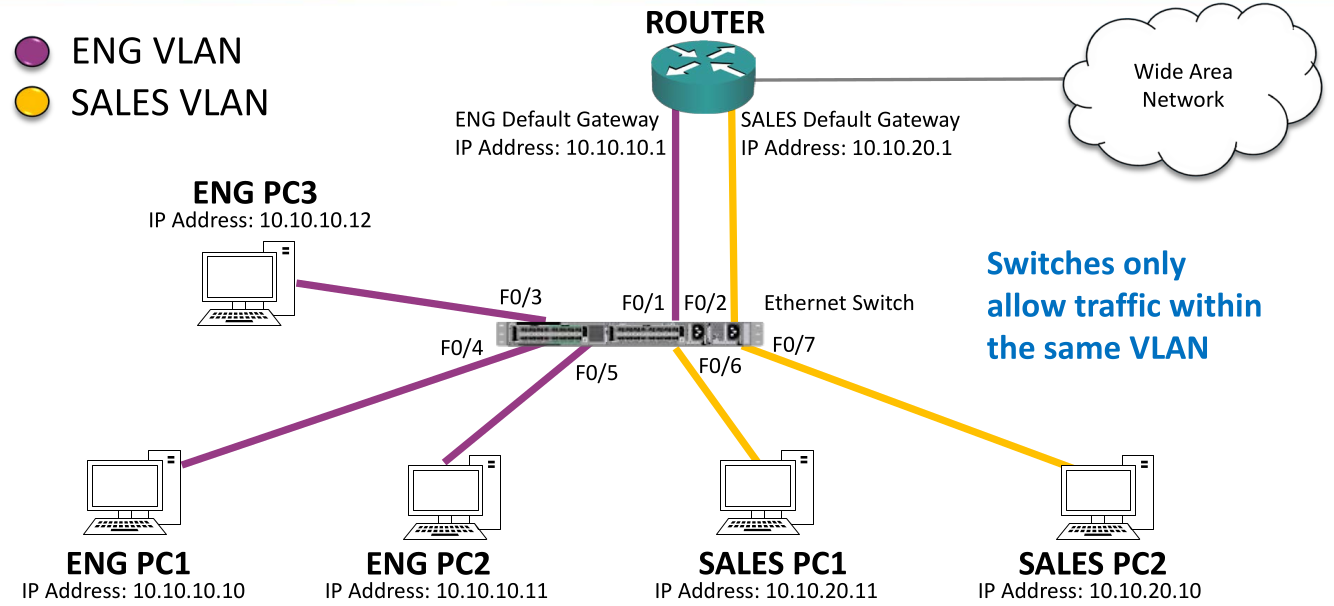
\includegraphics[width=\linewidth]{img/img14}
	\end{center}
\end{frame}

\begin{frame}
	\frametitle{Unicast Traffic within same IP subnet}
	\begin{center}
		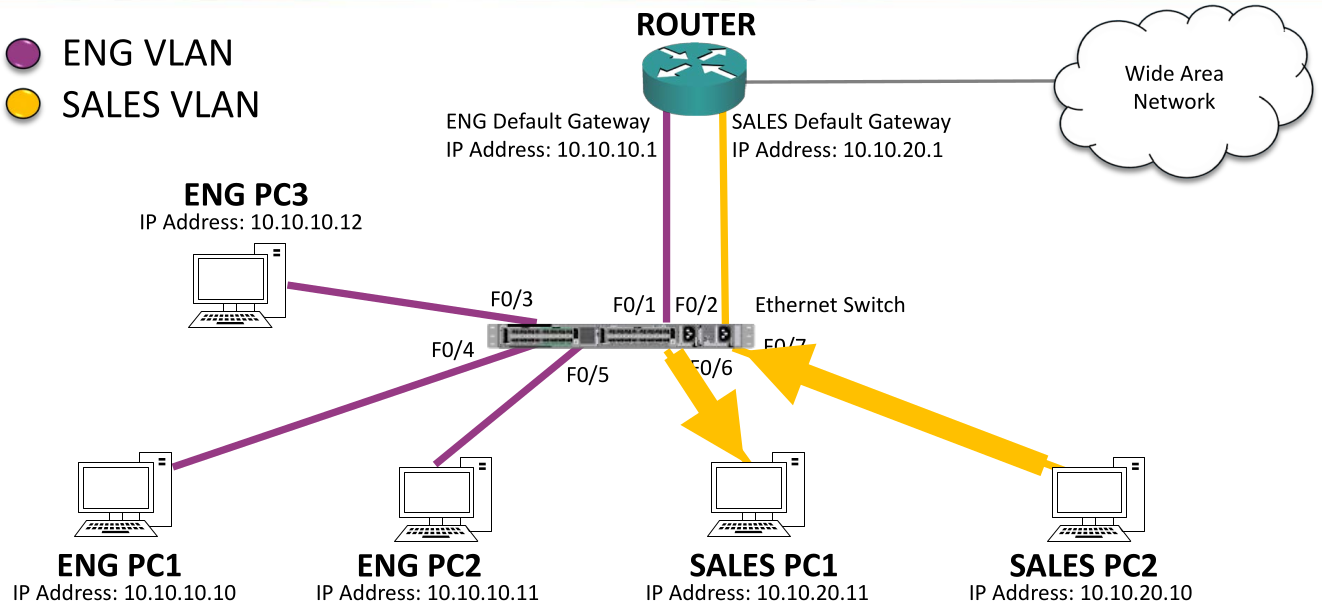
\includegraphics[width=\linewidth]{img/img15}
	\end{center}
\end{frame}

\begin{frame}
	\frametitle{Unicast Traffic between different IP subnets}
	\begin{center}
		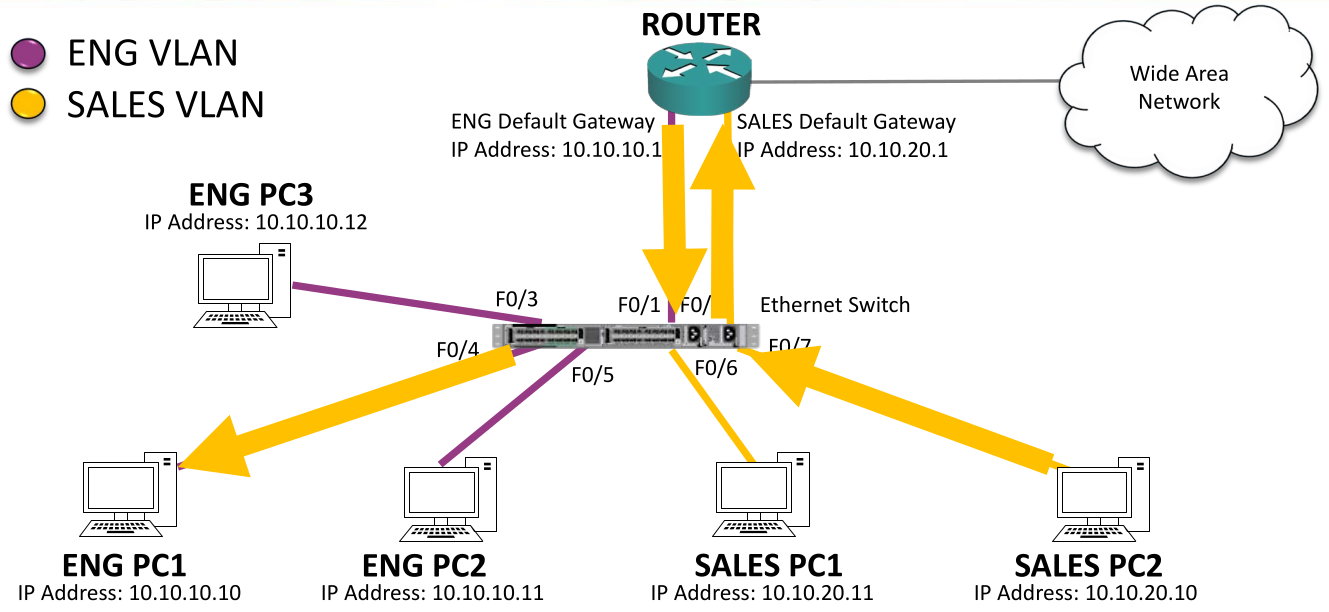
\includegraphics[width=\linewidth]{img/img16}
	\end{center}
\end{frame}

\begin{frame}
	\frametitle{Broadcast Traffic}
	\begin{center}
		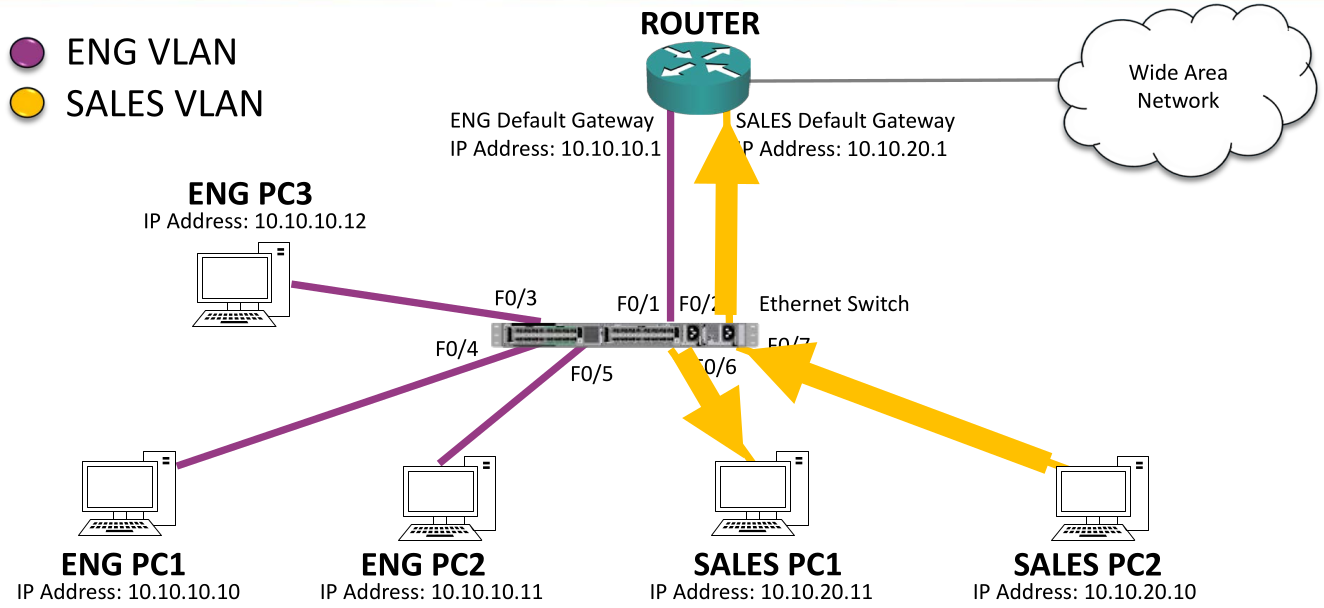
\includegraphics[width=\linewidth]{img/img17}
	\end{center}
\end{frame}

\section{VLAN Access Ports}

\begin{frame}
	\frametitle{VLAN Access Ports}
	\begin{center}
		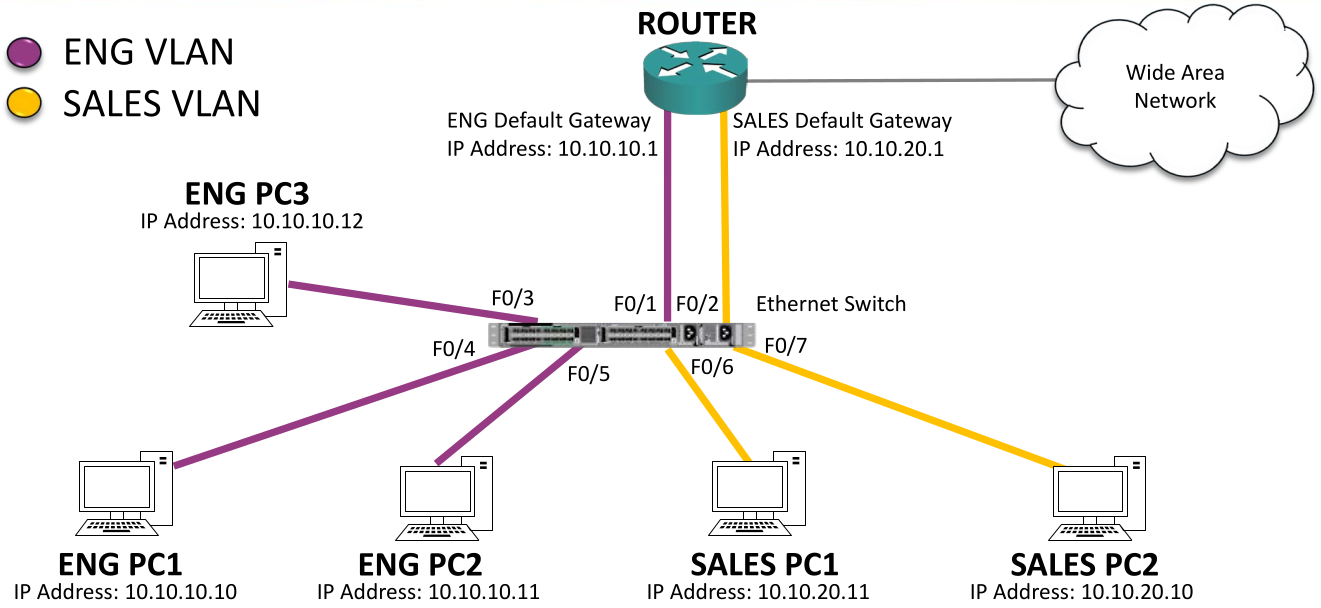
\includegraphics[width=\linewidth]{img/img18}
	\end{center}
\end{frame}

\begin{frame}
	\frametitle{What about the links between\\ switches?}
	\begin{center}
		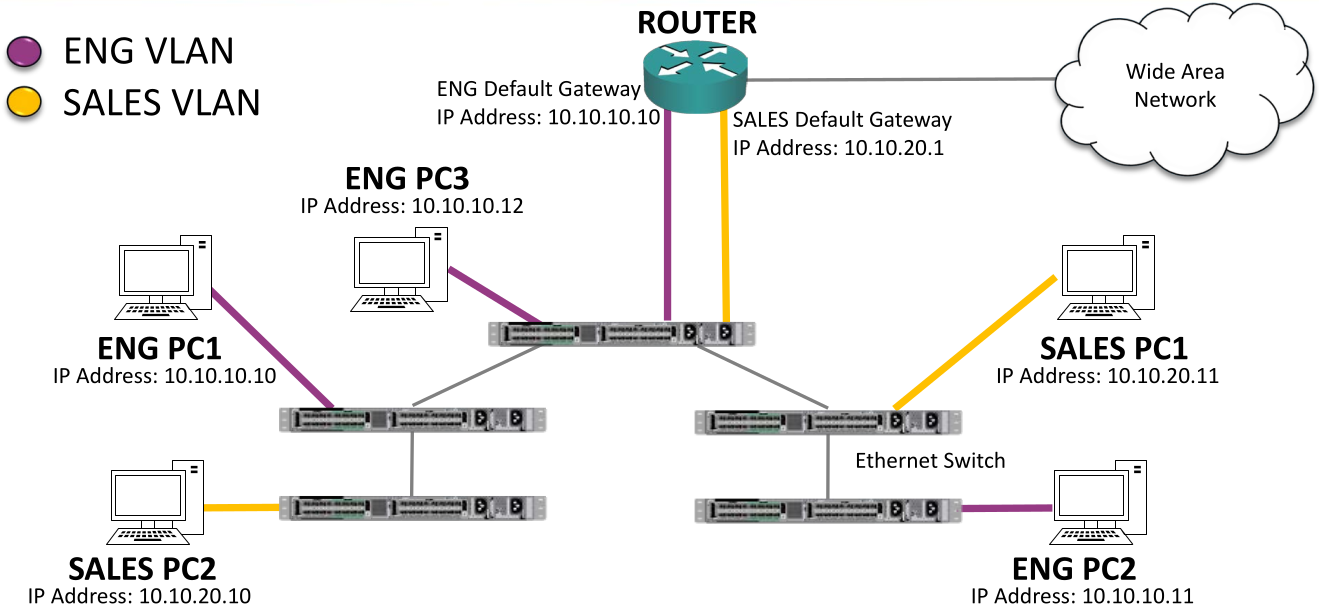
\includegraphics[width=\linewidth]{img/img19}
	\end{center}
\end{frame}

\begin{frame}{What about the links between\\ switches?}
	\begin{center}
		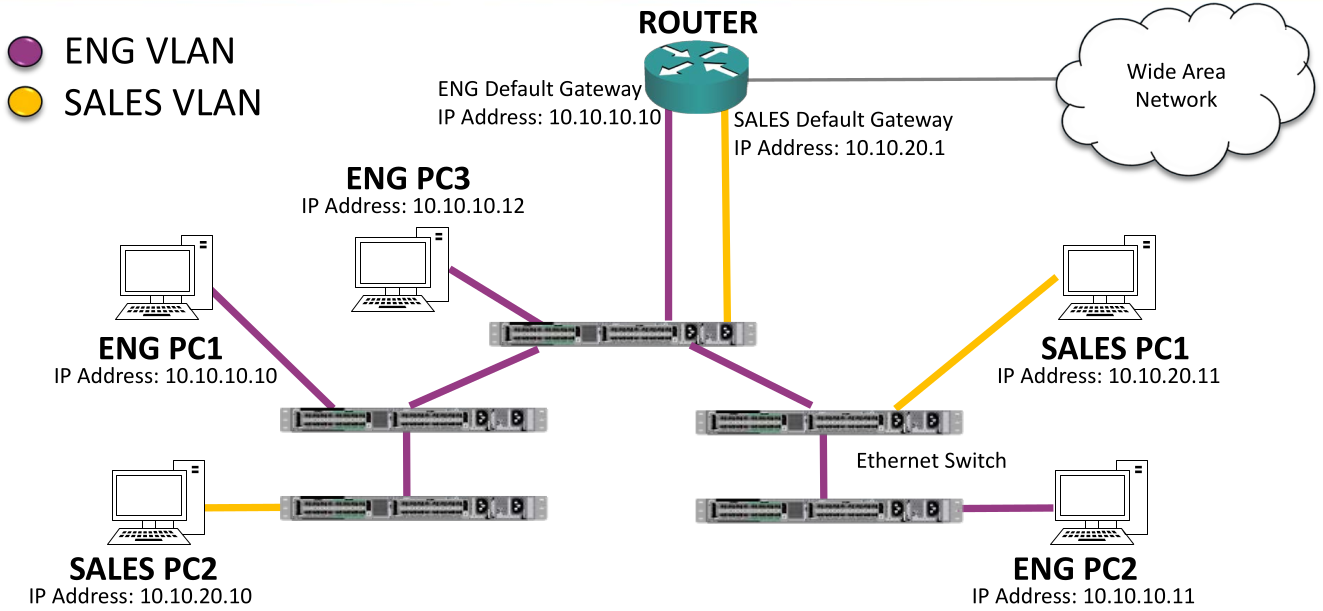
\includegraphics[width=\linewidth]{img/img20}
	\end{center}
\end{frame}

\begin{frame}
	\frametitle{Dot1Q Trunks}
	\begin{center}
		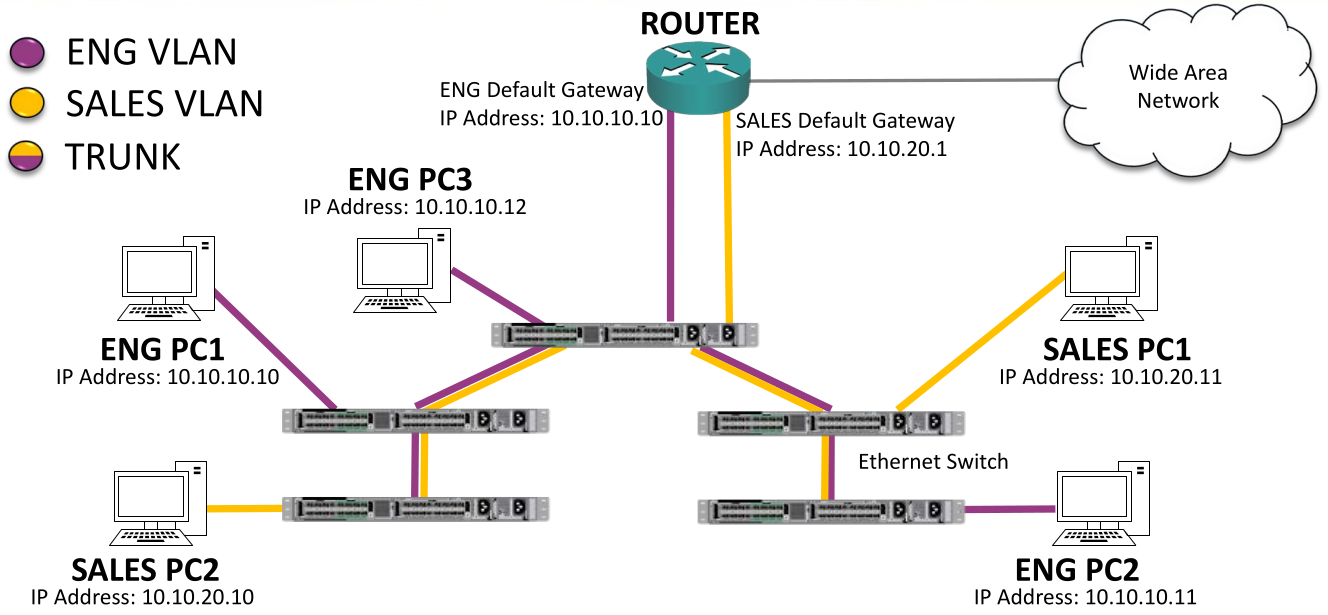
\includegraphics[width=\linewidth]{img/img21}
	\end{center}
\end{frame}

\begin{frame}{Dot1Q Trunks}
	\begin{itemize}
		\item An access port carries traffic for one specific VLAN
		\item Dot1Q trunks are configured on the links between switches where we
need to carry traffic for multiple VLANs
		\item ISL (Inter-Switch Link) was a Cisco proprietary trunking protocol which
is now obsolete
	\end{itemize}
\end{frame}

\begin{frame}{Dot1Q Trunks}
	\begin{itemize}
		\item When the switch forwards traffic to another switch, it tags the layer 2
Dot1Q header with the correct VLAN
		\item The receiving switch will only forward the traffic out ports that are in
that VLAN
		\item The switch removes the Dot1Q tag from the Ethernet frame when it
sends it to the end host
	\end{itemize}
\end{frame}

\begin{frame}{Dot1Q Trunks}
	\begin{center}
		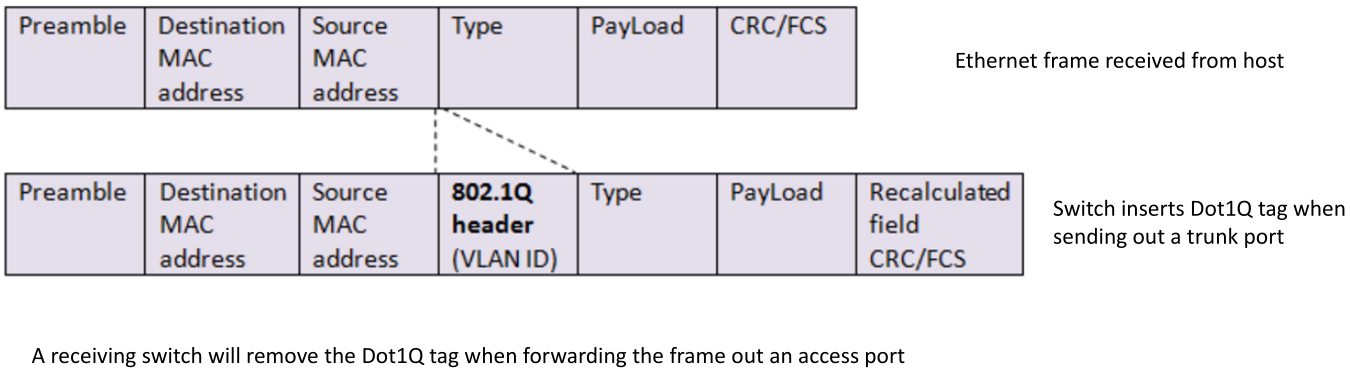
\includegraphics[width=\linewidth]{img/img22}
	\end{center}
\end{frame}

\begin{frame}{Dot1Q Trunks}
	\begin{center}
		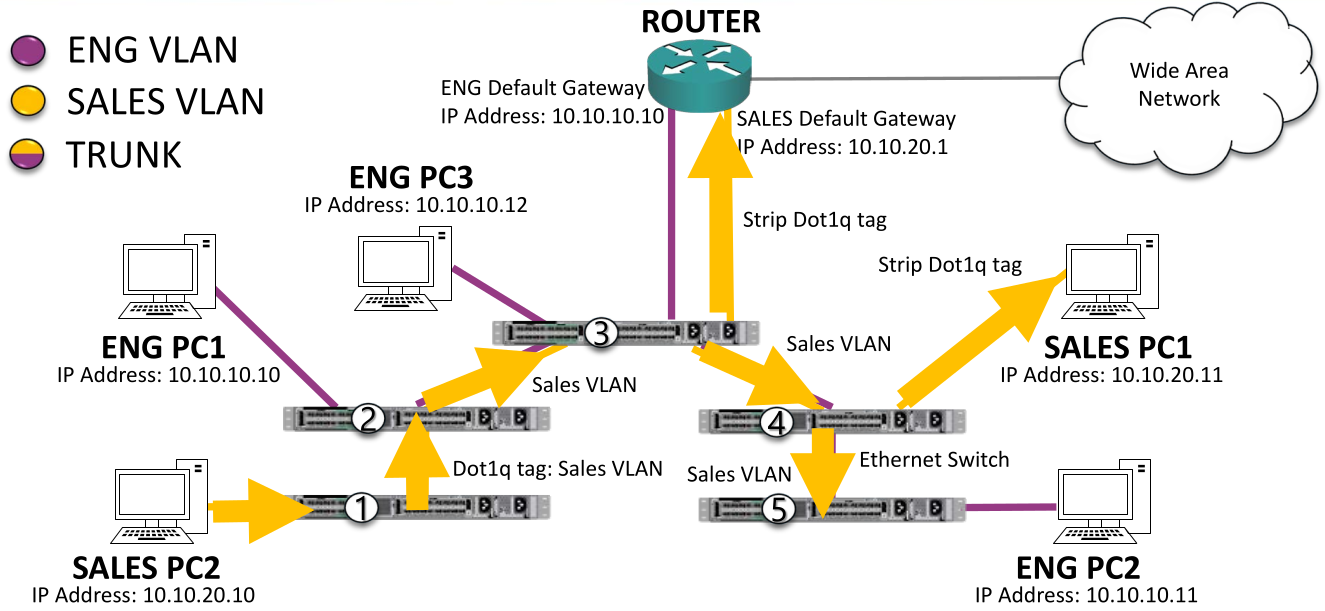
\includegraphics[width=\linewidth]{img/img23}
	\end{center}
\end{frame}

\begin{frame}
	\frametitle{Hypervisors - VLAN Aware Hosts}
	\begin{itemize}
		\item End hosts are typically members of only one VLAN and are not VLAN
aware
		\item A special case is virtualized hosts, where there are virtual machines in
different IP subnets on the host
		\item In this case we need to trunk the VLANs down to the host
	\end{itemize}
\end{frame}

\begin{frame}{Hypervisors - VLAN Aware Hosts}
	\begin{center}
		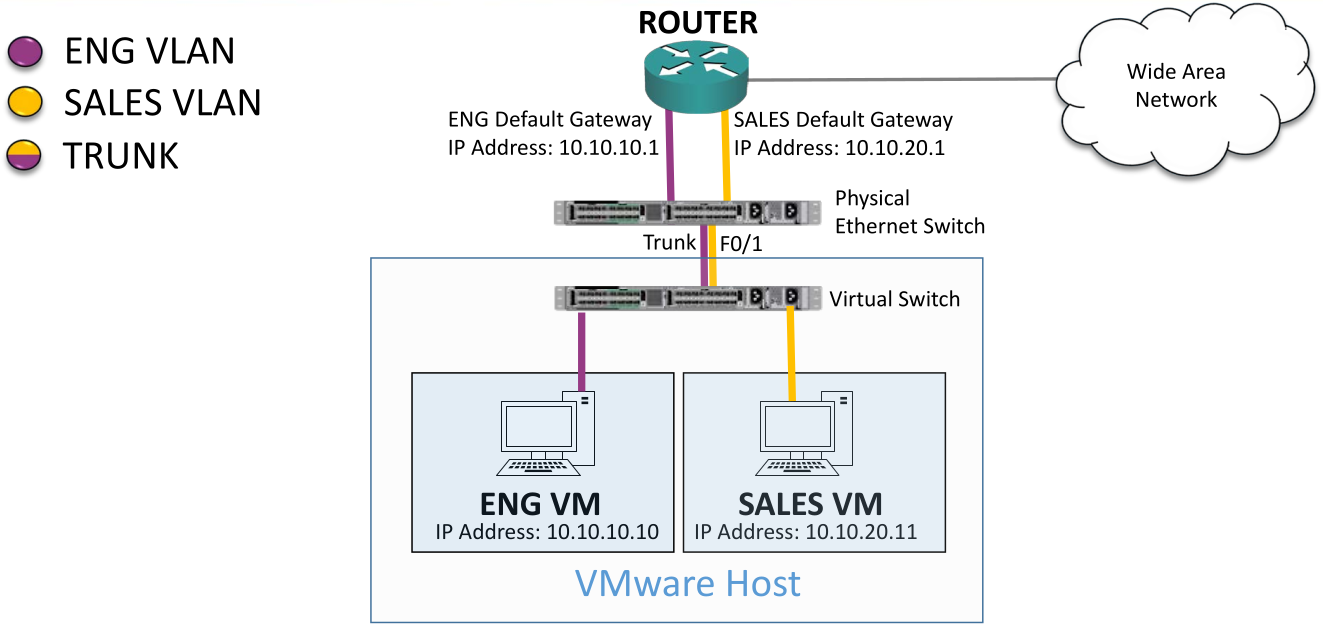
\includegraphics[width=\linewidth]{img/img24}
	\end{center}
\end{frame}

\begin{frame}
	\frametitle{Voice VLAN}
	\begin{center}
		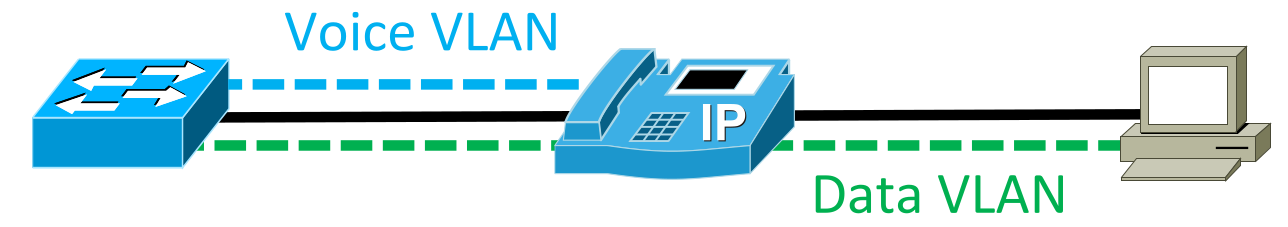
\includegraphics[width=\linewidth]{img/img25}
	\end{center}
\end{frame}

\begin{frame}
	\frametitle{Trunk Port Configuration}
	\begin{center}
		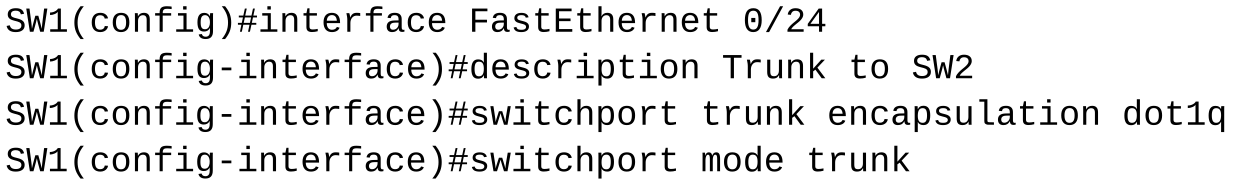
\includegraphics[width=\linewidth]{img/img26}
	\end{center}
\end{frame}

\begin{frame}
	\frametitle{Voice VLAN Configuration}
	\begin{center}
		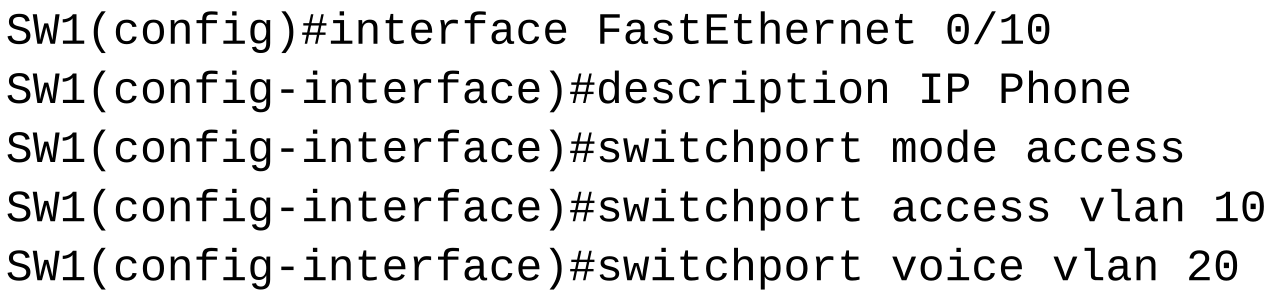
\includegraphics[width=\linewidth]{img/img27}
	\end{center}
\end{frame}

\begin{frame}
	\frametitle{The Native VLAN}
	\begin{itemize}
		\item The switch needs to know which VLAN to assign to any traffic which
comes in untagged on a trunk port
		\item This used to be required for when a switch was connected to a hub.
Hubs are Layer 1 devices so are not VLAN aware
		\item The Native VLAN is used for this
		\item The default Native VLAN is VLAN 1
		\item There are some security issues with using VLAN 1 as the Native VLAN so
best practice is to change it to an unused VLAN
		\item The Native VLAN must match on both sides of a trunk for it to come up
	\end{itemize}
\end{frame}

\begin{frame}
	\frametitle{Native VLAN Configuration}
	\begin{center}
		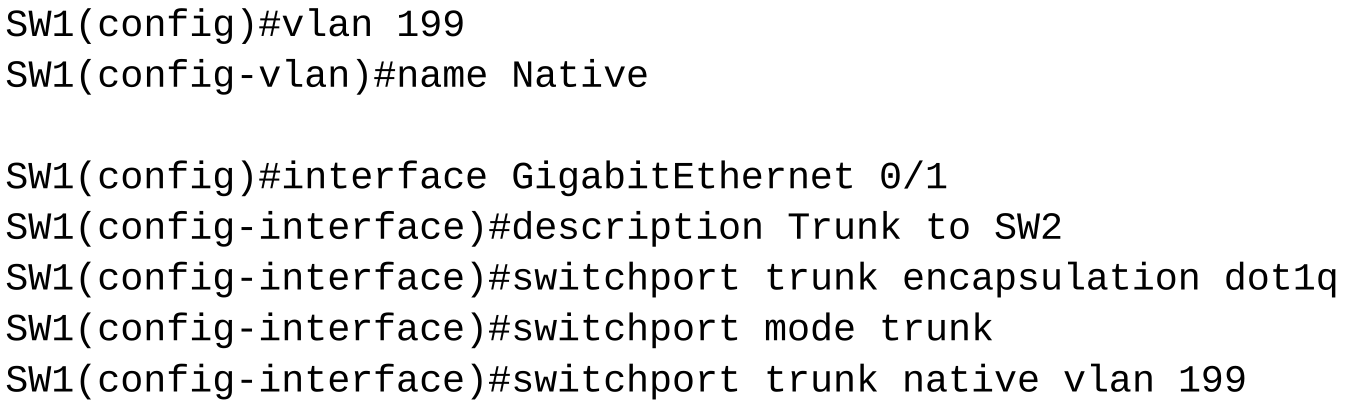
\includegraphics[width=\linewidth]{img/img28}
	\end{center}
\end{frame}

\begin{frame}
	\frametitle{Verification – show interface switchport}
	\begin{center}
		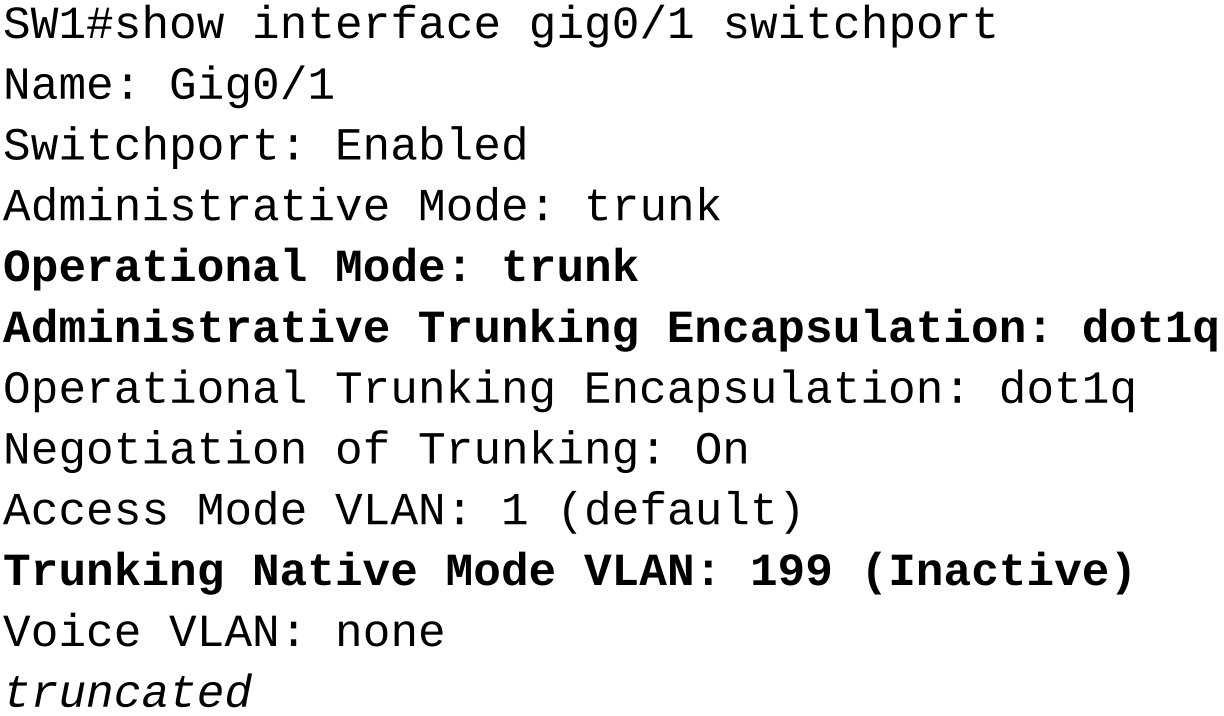
\includegraphics[width=\linewidth]{img/img29}
	\end{center}
\end{frame}

\begin{frame}
	\frametitle{Limiting Allowed VLANs}
	\begin{center}
		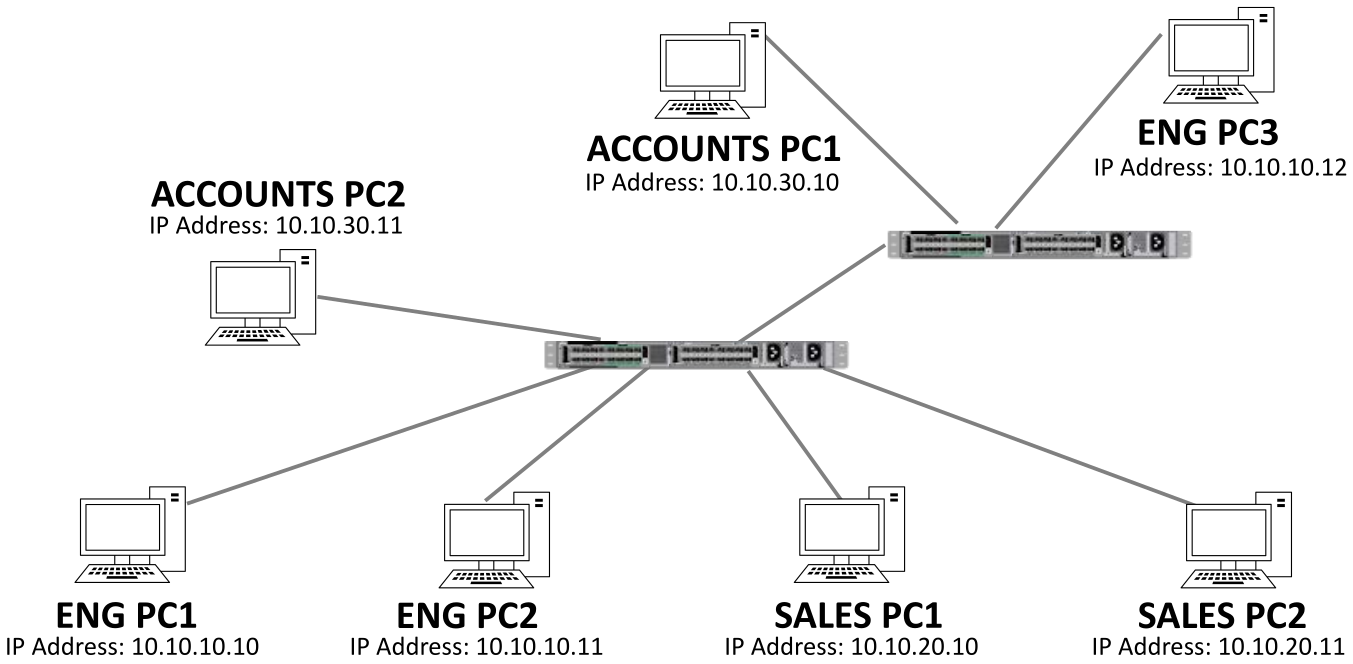
\includegraphics[width=\linewidth]{img/img30}
	\end{center}
\end{frame}

\begin{frame}
	\frametitle{Allowed VLAN Configuration}
	\begin{center}
		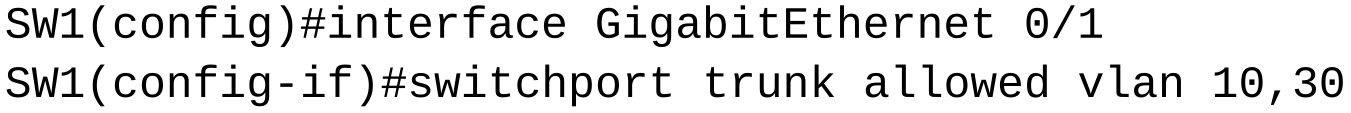
\includegraphics[width=\linewidth]{img/img31}
	\end{center}
\end{frame}

\begin{frame}
	\frametitle{VLAN Lab}
	\begin{center}
		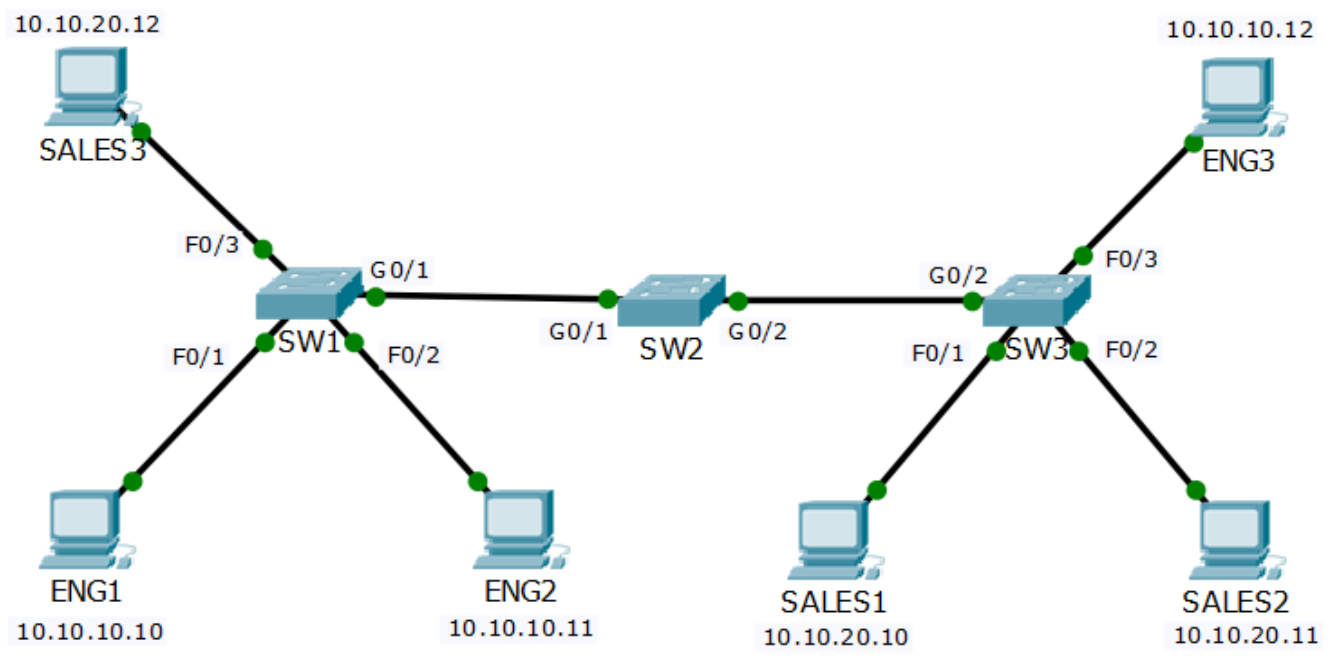
\includegraphics[width=\linewidth]{img/img32}
	\end{center}
\end{frame}

\section{VLAN Trunk Ports}

\section{DTP Dynamic Trunking Protocol}

\section{VTP VLAN Trunking Protocol}

\end{document}